\chapter{Kontextabgrenzung}
\label{ch:Kontextabgrenzung}
In der Kontextabgrenzung grenzen wir alle Kommunikationspartner vom System ab und stellen somit unsere externen Schnittstellen fest. Dazu wird der Kontext einerseits fachlich, als auch technisch voneinander abgegrenzt.
\section{Fachlicher Kontext}
Die fachliche Kontextabgrenzung dient uns dazu alle Kommunikationspartner zusammen mit den jeweiligen ein und Ausgabedaten mit dem System zu erläutern. Folgende Abbildung veranschaulicht die fachliche Kontextabgrenzung:
\begin{figure}[h]
	\centering
	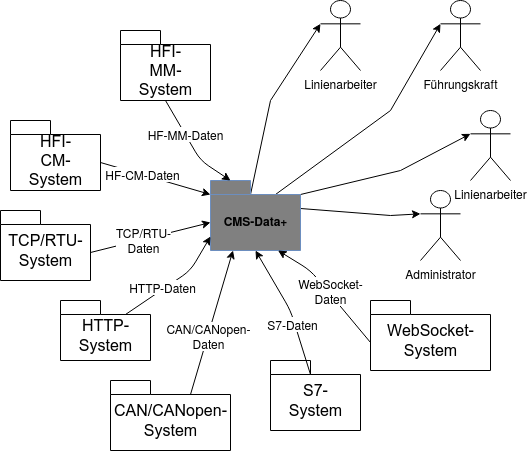
\includegraphics[width=0.6\textwidth]{Graphics/fachliche_kontextabgrenzung.png}
	\caption{Fachliche Kontextabgrenzung}
	\label{fig:fachliche_kontextabgrenzung}
\end{figure}

Wie das Diagramm veranschaulicht, dient das Data+ als Datensenke für alle angezeigten Systeme. Jedes dieser Systeme kann über eine eigene Schnittstelle bzw. Protokoll verfügen und über jenes die protokollspezifischen Daten an das Data+ senden.
Folgende Tabelle stellt noch einmal die Kommunikationspartner und den fachlichen Kontext zum System dar:

\begin{table}[t]
	\begin{tabularx}{\textwidth}{|p{3cm}|X|X|}
		\hline
		Kommunikations-
		partner & Eingabe & Ausgabe \\
		\hline
		HFI-MM-System & & \\
		\hline
		HFI-CM-System & & \\
		\hline
		TCP/RTU-System & & \\
		\hline
		HTTP-
		System & & \\
		\hline
		CAN/CANopen-
		System & & \\
		\hline
		S7-System & & \\
		\hline
		WebSocket-System & & \\
		\hline
	\end{tabularx} 
	\caption{Fachliche Kontextabgrenzung der Kommunikationspartner}
	\label{tab:FachlicheKontextabgrenzungDerKommunikationspartner}
\end{table}

\section{Technischer Kontext}
Der technische Kontext definiert die Kanäle und das Übertragungsmedium über dem unser System mit externen Komponenten interagiert. Dabei wird erklärt, wie und über welche technischen Kanäle unsere fachlichen Ein- und Ausgaben ablaufen. Zur Veranschaulichung wird dies im folgenden UML Deployment-Diagramm dargestellt:

\begin{figure}[h]
	\centering
	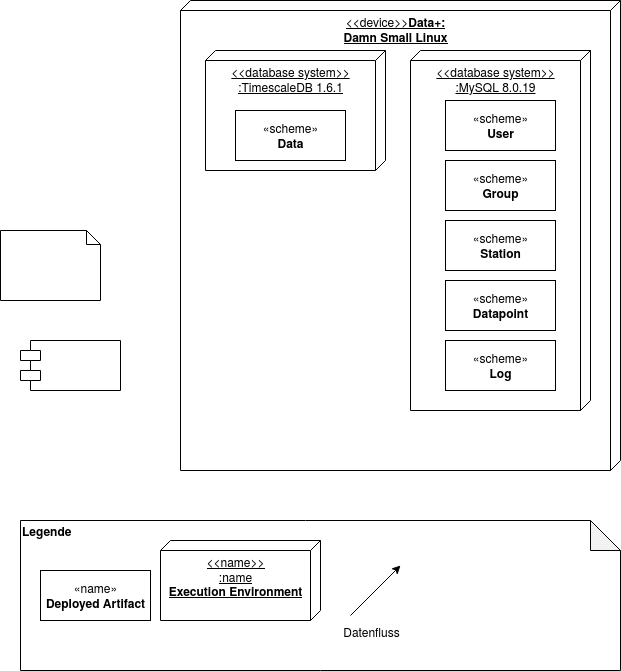
\includegraphics[width=0.6\textwidth]{Graphics/technische_kontextabgrenzung.png}
	\caption{Technische Kontextabgrenzung}
	\label{fig:technische_kontextabgrenzung}
\end{figure}